\chapter{Pola Struktural (Bagian 1)}


Pola struktural dalam rekayasa perangkat lunak berorientasi objek berfokus pada cara menyusun kelas dan objek untuk membentuk struktur yang lebih besar dan fleksibel. Pola-pola ini dirancang untuk memastikan bahwa komponen dalam sistem dapat berinteraksi secara efisien, terlepas dari kompleksitas atau perbedaan antarmuka yang ada. Dalam bab ini, dibahas beberapa pola struktural yang umum digunakan, yaitu \textit{Adapter}, \textit{Decorator}, \textit{Bridge}, dan \textit{Composite}, lengkap dengan tujuan, studi kasus, kelebihan, kekurangan, dan contoh implementasi dalam Java.


\section{Adapter}

\subsection{Tujuan dan Konteks Penggunaan}

Pola \textit{Adapter} adalah salah satu pola struktural yang bertujuan untuk menjembatani dua antarmuka yang tidak kompatibel, sehingga kelas yang tidak bisa bekerja sama secara langsung dapat berinteraksi tanpa perlu mengubah kode aslinya. Pola ini menciptakan lapisan perantara (\textit{wrapper}) yang mengubah antarmuka dari sebuah kelas menjadi antarmuka lain yang diharapkan oleh klien.

Tujuan utama dari pola Adapter adalah untuk mengintegrasikan sistem yang sudah ada (legacy systems) atau pustaka pihak ketiga ke dalam sistem baru tanpa memodifikasi kode sumber aslinya. Dengan menggunakan adapter, kita dapat memastikan bahwa kelas dengan antarmuka berbeda tetap dapat dimanfaatkan dengan antarmuka yang diinginkan klien.

Pola Adapter sangat relevan digunakan ketika:
\begin{itemize}
	\item Kita ingin menggunakan kelas pihak ketiga, tetapi antarmukanya tidak sesuai dengan sistem yang kita miliki.
	\item Sistem telah dikembangkan dalam waktu lama, namun perlu beradaptasi dengan antarmuka baru tanpa refactor besar-besaran.
	\item Kita ingin memisahkan kode klien dari detail implementasi atau struktur asli dari kelas atau sistem yang digunakan.
\end{itemize}

Secara umum, adapter bekerja seperti konektor antarmuka: klien tetap menggunakan antarmuka yang ia kenali (\texttt{Target}), sedangkan adapter meneruskan permintaan tersebut ke antarmuka asli yang berbeda milik \texttt{Adaptee}. Ini memungkinkan penggunaan kembali kode tanpa perlu mengubah kode sumber atau antarmuka klien.

Pola Adapter sering dijumpai dalam:
\begin{itemize}
	\item Integrasi antarmuka pemrograman aplikasi (API) eksternal ke dalam sistem internal.
	\item Sistem antarmuka pengguna (GUI) yang ingin memanfaatkan komponen visual dari pustaka lain.
	\item Sistem berbasis perangkat keras atau protokol komunikasi yang berbeda, seperti konversi antara port USB dan serial.
\end{itemize}

Dengan menerapkan pola Adapter, sistem menjadi lebih fleksibel, mudah diperluas, dan lebih tahan terhadap perubahan struktur dari pustaka luar atau sistem lama yang sulit diubah.

\subsection{Contoh Kasus Penggunaan}

Salah satu contoh klasik penggunaan pola \textit{Adapter} adalah ketika sebuah aplikasi modern perlu menggunakan pustaka atau modul lama (legacy) yang memiliki antarmuka berbeda. Misalnya, dalam pengembangan perangkat lunak modern, pengembang mungkin ingin menggunakan kelas lama yang menyediakan data dalam format XML, sedangkan sistem baru membutuhkan data dalam format JSON. Untuk menjembatani perbedaan ini tanpa memodifikasi kelas lama, pengembang dapat membuat sebuah adapter yang mengonversi hasil dari kelas lama (XML) ke dalam bentuk JSON yang diharapkan.

Contoh lainnya adalah dalam pengembangan antarmuka pengguna (UI), di mana framework baru seperti JavaFX ingin menggunakan komponen dari Swing. Karena JavaFX dan Swing memiliki struktur antarmuka yang berbeda, adapter diperlukan untuk membungkus komponen Swing sehingga dapat digunakan dalam konteks JavaFX tanpa harus menulis ulang seluruh komponen dari awal.

Di dunia perangkat keras dan protokol komunikasi, adapter sangat lazim. Sebagai contoh, konektor USB-to-Serial adalah adapter fisik yang mengubah protokol komunikasi dari USB ke RS-232 agar perangkat lama dapat tetap digunakan di komputer modern. Pola yang sama berlaku dalam perangkat lunak ketika dua sistem perlu berkomunikasi tetapi menggunakan protokol atau format data yang berbeda.

Contoh tambahan dalam pengembangan aplikasi web adalah ketika sebuah sistem e-commerce ingin mengintegrasikan layanan pembayaran dari berbagai penyedia (misalnya PayPal, Stripe, dan bank lokal), tetapi masing-masing memiliki API berbeda. Dengan membuat adapter untuk setiap penyedia, sistem e-commerce cukup berinteraksi dengan satu antarmuka standar (\texttt{PaymentGateway}), sementara detail teknis masing-masing penyedia disembunyikan oleh adapter mereka.

\textbf{Contoh dalam praktik:}
\begin{itemize}
	\item Dalam pustaka grafik, adapter digunakan untuk mengintegrasikan objek gambar dari format atau sumber berbeda (misalnya dari BufferedImage ke Image).
	\item Saat menggunakan API Android lama dengan arsitektur baru berbasis MVVM, adapter dibutuhkan untuk menyelaraskan View lama dengan ViewModel modern.
	\item Dalam pengembangan REST API, adapter dapat digunakan untuk menerjemahkan permintaan API publik ke dalam pemanggilan metode internal sistem mikroservis yang memiliki kontrak berbeda.
\end{itemize}

Dengan pola \textit{Adapter}, sistem menjadi lebih tangguh terhadap perubahan antarmuka eksternal dan dapat mempertahankan kompatibilitas dengan komponen lama tanpa mengorbankan struktur internal aplikasi yang modern dan terstandarisasi.

\subsection{Kelebihan dan Kekurangan}

Pola \textit{Adapter} menawarkan berbagai keuntungan dalam pengembangan perangkat lunak, terutama dalam hal kompatibilitas dan penggunaan kembali komponen. Namun, seperti pola desain lainnya, penggunaan Adapter juga memiliki keterbatasan yang perlu dipertimbangkan sebelum diterapkan dalam sebuah sistem.

\textbf{Kelebihan:}
\begin{itemize}
	\item \textbf{Meningkatkan kompatibilitas antar sistem:} Adapter memungkinkan dua kelas atau sistem yang memiliki antarmuka berbeda untuk bekerja sama tanpa memodifikasi kode aslinya. Ini sangat bermanfaat dalam integrasi sistem lama dengan sistem baru.
	
	\item \textbf{Mendukung prinsip Open/Closed:} Kode adaptee dan klien tidak perlu diubah. Perubahan hanya dilakukan dengan menambahkan adapter, sehingga kode terbuka untuk ekstensi namun tertutup untuk modifikasi.
	
	\item \textbf{Mempermudah penggunaan kembali kode:} Dengan menggunakan adapter, kita dapat menggunakan kembali kelas yang sudah ada walaupun antarmukanya berbeda dari yang diharapkan, tanpa perlu menyalin atau menulis ulang logika internalnya.
	
	\item \textbf{Meningkatkan fleksibilitas:} Adapter dapat digunakan untuk menyatukan banyak kelas yang tidak kompatibel namun memiliki perilaku serupa, dengan menyatukan mereka di bawah antarmuka yang sama.
	
	\item \textbf{Menyederhanakan integrasi pihak ketiga:} Saat menggunakan pustaka eksternal yang tidak bisa diubah, adapter menyediakan solusi yang bersih untuk menyelaraskan antarmuka eksternal dengan sistem internal.
\end{itemize}

\textbf{Kekurangan:}
\begin{itemize}
	\item \textbf{Menambah lapisan kompleksitas:} Penggunaan adapter menambah satu lapisan tambahan dalam arsitektur sistem. Jika tidak dikelola dengan baik, ini dapat membuat struktur kode menjadi lebih sulit dilacak atau dipahami.
	
	\item \textbf{Berpotensi menyembunyikan kekacauan desain:} Adapter dapat digunakan untuk menyamarkan atau menambal ketidaksesuaian desain yang seharusnya diatasi melalui refaktor menyeluruh. Ini bisa memperpanjang umur kode yang sebenarnya perlu diperbaiki.
	
	\item \textbf{Kinerja sedikit menurun:} Meskipun tidak signifikan, penggunaan adapter menambahkan overhead pemanggilan metode tambahan, terutama jika digunakan dalam sistem dengan performa tinggi atau panggilan berulang.
	
	\item \textbf{Sulit dikelola jika terlalu banyak adapter:} Dalam sistem besar dengan banyak variasi antarmuka, jumlah adapter bisa menjadi banyak dan sulit dikelola, apalagi jika masing-masing adapter memiliki perilaku yang berbeda-beda.
	
	\item \textbf{Tidak selalu cocok untuk semua jenis perbedaan:} Jika perbedaan antara antarmuka sangat mendasar atau mencakup banyak aspek semantik, adapter bisa menjadi solusi yang terlalu sempit dan tidak efisien dibandingkan pendekatan arsitektur ulang.
\end{itemize}

Dengan mempertimbangkan kelebihan dan kekurangan di atas, pola \textit{Adapter} sebaiknya digunakan secara selektif—terutama saat menghadapi integrasi antara sistem lama dan baru, atau saat menyatukan berbagai pustaka dengan antarmuka berbeda dalam satu sistem yang konsisten dan terstruktur.

\subsection{Implementasi dalam Java}

Implementasi pola \textit{Adapter} dalam Java dapat dilakukan dengan dua pendekatan utama, yaitu menggunakan pewarisan (\textit{class adapter}) atau menggunakan komposisi (\textit{object adapter}). Pendekatan yang paling umum dan fleksibel adalah menggunakan komposisi, karena Java tidak mendukung pewarisan ganda (multiple inheritance) secara langsung.

Gambar~\ref{fig:adapter} menunjukkan struktur pola \textit{Adapter} dalam bentuk diagram UML. Dalam diagram tersebut, \texttt{Client} berinteraksi dengan \texttt{Target} interface, yang kemudian diimplementasikan oleh \texttt{Adapter}. \texttt{Adapter} secara internal memanggil metode-metode pada kelas \texttt{Adaptee} untuk menyediakan perilaku yang sesuai dengan antarmuka \texttt{Target}.

\begin{figure}[h]
	\centering
	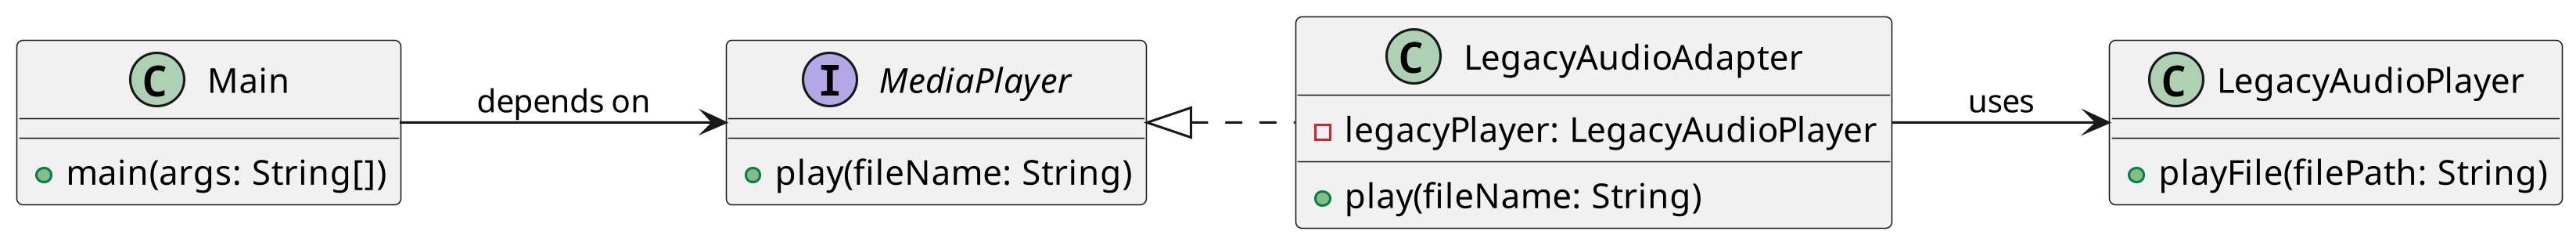
\includegraphics[width=\textwidth]{../figures/out/adapter.png}
	\caption{Struktur Pola Adapter}
	\label{fig:adapter}
\end{figure}

Berikut adalah contoh implementasi pola \textit{Adapter} menggunakan pendekatan \textit{object adapter} di Java. Studi kasus ini menggunakan contoh di mana sebuah sistem modern mengharapkan antarmuka \texttt{MediaPlayer}, sementara kelas lama menggunakan antarmuka berbeda bernama \texttt{LegacyAudioPlayer}.

\begin{lstlisting}[style=JavaStyle, caption={Interface Target: MediaPlayer}, label={lst:adapter-target}]
	public interface MediaPlayer {
		void play(String fileName);
	}
\end{lstlisting}

\begin{lstlisting}[style=JavaStyle, caption={Kelas Legacy (Adaptee): LegacyAudioPlayer}, label={lst:adapter-adaptee}]
	public class LegacyAudioPlayer {
		public void playFile(String filePath) {
			System.out.println("Playing file from legacy player: " + filePath);
		}
	}
\end{lstlisting}

\begin{lstlisting}[style=JavaStyle, caption={Adapter: LegacyAudioAdapter}, label={lst:adapter-adapter}]
	public class LegacyAudioAdapter implements MediaPlayer {
		private LegacyAudioPlayer legacyPlayer;
		
		public LegacyAudioAdapter(LegacyAudioPlayer legacyPlayer) {
			this.legacyPlayer = legacyPlayer;
		}
		
		@Override
		public void play(String fileName) {
			// Mengalihkan permintaan ke metode dari LegacyAudioPlayer
			legacyPlayer.playFile(fileName);
		}
	}
\end{lstlisting}

\begin{lstlisting}[style=JavaStyle, caption={Client: Menggunakan Adapter}, label={lst:adapter-client}]
	public class Main {
		public static void main(String[] args) {
			MediaPlayer player = new LegacyAudioAdapter(new LegacyAudioPlayer());
			player.play("music.mp3");
		}
	}
\end{lstlisting}

Dalam contoh di atas, antarmuka \texttt{MediaPlayer} didefinisikan sebagai kontrak umum yang diharapkan oleh klien. Kelas lama \texttt{LegacyAudioPlayer} memiliki antarmuka yang berbeda, yaitu metode \texttt{playFile(String)}. Untuk menjembatani keduanya, dibuatlah kelas adapter bernama \texttt{LegacyAudioAdapter} yang mengimplementasikan \texttt{MediaPlayer} dan menggunakan komposisi untuk memanggil metode dari \texttt{LegacyAudioPlayer}.

Ketika objek adapter digunakan oleh klien, ia akan memanggil metode \texttt{play()} dari \texttt{MediaPlayer}, dan adapter akan menerjemahkan permintaan tersebut ke metode \texttt{playFile()} milik kelas lama. Dengan cara ini, integrasi berhasil dilakukan tanpa memodifikasi kode lama maupun kode klien.

Pendekatan ini menjadikan sistem lebih modular dan fleksibel, karena berbagai jenis \texttt{Adaptee} dapat diintegrasikan hanya dengan menulis adapter baru yang sesuai dengan antarmuka \texttt{Target} yang sama.



\section{Decorator}

\subsection{Tujuan dan Konteks Penggunaan}

Pola \textit{Decorator} adalah salah satu pola struktural yang bertujuan untuk menambahkan tanggung jawab atau perilaku baru ke sebuah objek secara dinamis, tanpa harus memodifikasi kode kelas aslinya. Pola ini memungkinkan ekstensi fungsionalitas objek secara fleksibel melalui pembungkusan (wrapping) menggunakan kelas lain yang disebut \texttt{Decorator}, yang memiliki antarmuka yang sama dengan objek yang dibungkus.

Tujuan utama dari pola Decorator adalah untuk mengatasi keterbatasan pewarisan tunggal dalam bahasa seperti Java, dengan menyediakan alternatif terhadap pewarisan untuk memperluas perilaku objek. Dengan pendekatan ini, pengembang dapat menambahkan fitur baru pada objek tertentu tanpa memengaruhi objek lain dari kelas yang sama.

Pola ini sangat berguna ketika:
\begin{itemize}
	\item Diperlukan penambahan fitur tambahan secara selektif ke objek tertentu, tanpa mempengaruhi semua instansi dari kelas tersebut.
	\item Sistem menghindari penggunaan pewarisan yang dalam atau kompleks, karena dapat menyebabkan rigiditas dan sulit dirawat.
	\item Perilaku tambahan perlu ditambahkan secara berlapis-lapis, di mana tiap lapisan bertanggung jawab atas satu fungsi tambahan tertentu.
\end{itemize}

Contoh umum penggunaan Decorator dapat ditemukan dalam pengembangan antarmuka pengguna (GUI), di mana komponen visual seperti tombol dapat dibungkus dengan decorator yang menambahkan border, scrollbar, atau efek bayangan. Alih-alih membuat banyak subclass seperti \texttt{ScrollableBorderedButtonWithShadow}, pola decorator memungkinkan komposisi perilaku yang fleksibel.

Selain itu, pola ini juga sering digunakan dalam pengembangan sistem input/output seperti \texttt{java.io} di Java, di mana objek seperti \texttt{BufferedReader}, \texttt{InputStreamReader}, dan \texttt{FileReader} membungkus satu sama lain untuk menambahkan fitur pembacaan baris, konversi karakter, atau pembacaan file.

Pola ini mendukung prinsip desain perangkat lunak modern seperti:
\begin{itemize}
	\item \textbf{Open/Closed Principle:} Kelas terbuka untuk diperluas, tetapi tertutup untuk diubah.
	\item \textbf{Single Responsibility Principle:} Setiap decorator dapat memiliki satu tanggung jawab tambahan secara terpisah.
\end{itemize}

Dengan pola \textit{Decorator}, sistem menjadi lebih modular dan mudah disesuaikan karena fitur tambahan dapat dirangkai sesuai kebutuhan, tanpa membebani kelas dasar dengan semua kemungkinan variasi perilaku.

\subsection{Contoh Kasus Penggunaan}

Pola \textit{Decorator} sangat efektif ketika kita ingin menambahkan perilaku tambahan pada objek tertentu tanpa memengaruhi seluruh kelas atau objek lain dari kelas yang sama. Hal ini membuat pola ini ideal untuk digunakan dalam konteks di mana fleksibilitas dan modularitas tinggi diperlukan dalam pengembangan fitur.

Salah satu contoh paling umum ditemukan dalam pengembangan antarmuka pengguna (UI). Misalnya, dalam sebuah aplikasi desktop, komponen dasar seperti \texttt{TextField} dapat dihias (decorated) dengan berbagai fitur tambahan, seperti penambahan border, scrollbar, ikon validasi, atau efek animasi. Dengan menggunakan decorator, pengembang dapat membuat kombinasi fitur-fitur ini tanpa harus membuat subclass baru untuk setiap kombinasi. Sebagai contoh, daripada membuat kelas seperti \texttt{BorderedScrollableTextFieldWithTooltip}, kita cukup membungkus \texttt{TextField} dengan serangkaian decorator seperti \texttt{BorderDecorator}, \texttt{ScrollDecorator}, dan \texttt{TooltipDecorator}.

Contoh lainnya dapat ditemukan pada pustaka \texttt{java.io} di Java, yang menerapkan pola decorator secara ekstensif untuk menangani input dan output. Objek dasar seperti \texttt{InputStream} dapat dihias dengan \texttt{BufferedInputStream} untuk memberikan fitur buffering, atau dengan \texttt{DataInputStream} untuk membaca tipe data primitif dari stream. Hal ini memungkinkan pembuatan rantai decorator yang fleksibel seperti:

\begin{lstlisting}[style=JavaStyle]
	InputStream input = new BufferedInputStream(new FileInputStream("data.txt"));
\end{lstlisting}

Contoh lain adalah dalam sistem notifikasi. Sebuah objek \texttt{Notifier} dapat didekorasi dengan lapisan tambahan seperti \texttt{EmailNotifier}, \texttt{SMSNotifier}, atau \texttt{SlackNotifier}, sehingga notifikasi dapat dikirim ke berbagai kanal tanpa memodifikasi logika dasar notifikasi. Setiap lapisan decorator dapat menambahkan media pengiriman tertentu secara terpisah.

Dalam pengembangan game, pola decorator digunakan untuk menambahkan kemampuan atau atribut sementara pada karakter permainan. Misalnya, karakter \texttt{Player} dapat dihias dengan \texttt{ShieldDecorator} untuk menambah pertahanan, atau \texttt{SpeedBoostDecorator} untuk meningkatkan kecepatan selama beberapa detik.

\textbf{Contoh dalam praktik:}
\begin{itemize}
	\item Sistem pengamanan HTTP request, di mana request dapat dibungkus dengan decorator yang menambahkan otentikasi, logging, atau validasi input secara bertingkat.
	\item Dalam rendering teks, decorator dapat menambahkan efek seperti tebal, miring, garis bawah, atau warna tertentu ke elemen teks.
	\item Sistem keuangan, di mana transaksi dasar dihias dengan decorator seperti \texttt{AuditDecorator}, \texttt{LoggingDecorator}, atau \texttt{ValidationDecorator} untuk menambahkan fungsi secara modular.
\end{itemize}

Pola decorator memberikan fleksibilitas tinggi dalam membangun perilaku objek secara bertahap, tanpa menciptakan struktur pewarisan yang kaku dan tidak scalable. Hal ini menjadikannya sangat cocok untuk sistem yang berkembang dan terus membutuhkan variasi fitur atau perilaku tambahan secara selektif.

\subsection{Kelebihan dan Kekurangan}

Pola \textit{Decorator} memiliki sejumlah keunggulan yang menjadikannya pilihan utama dalam berbagai situasi di mana perluasan perilaku objek harus dilakukan secara fleksibel dan tanpa memengaruhi struktur kode yang ada. Namun demikian, seperti pola desain lainnya, pola ini juga memiliki beberapa kekurangan yang perlu diperhatikan sebelum diterapkan dalam sistem nyata.

\textbf{Kelebihan:}
\begin{itemize}
	\item \textbf{Memperluas fungsionalitas tanpa mengubah kelas asli:} Dengan pola decorator, kita dapat menambahkan fitur tambahan ke objek tertentu tanpa mengubah kode sumber dari kelas utama atau kelas lain yang menggunakan objek tersebut.
	
	\item \textbf{Mendukung komposisi dibanding pewarisan:} Pola ini mendorong penggunaan komposisi objek, yang lebih fleksibel dan scalable dibanding pewarisan, terutama dalam sistem dengan banyak kemungkinan kombinasi fitur.
	
	\item \textbf{Mendukung prinsip Open/Closed:} Kelas terbuka untuk diperluas namun tertutup untuk diubah. Decorator memungkinkan pengembang untuk menambahkan fungsionalitas baru tanpa menyentuh kode kelas yang sudah ada.
	
	\item \textbf{Mendukung Single Responsibility Principle:} Setiap decorator memiliki satu tanggung jawab tambahan, sehingga perubahan dalam satu aspek tidak memengaruhi aspek lain dalam sistem.
	
	\item \textbf{Fleksibel dan dapat dikombinasikan secara bertingkat:} Beberapa decorator dapat digunakan secara bersamaan dalam satu objek, memungkinkan perilaku objek dibangun secara bertahap dan modular.
\end{itemize}

\textbf{Kekurangan:}
\begin{itemize}
	\item \textbf{Struktur kode bisa menjadi kompleks:} Ketika banyak decorator digunakan secara bertingkat, akan sulit untuk memahami aliran logika dan urutan eksekusi, terutama bagi pengembang baru dalam proyek.
	
	\item \textbf{Sulit dalam debugging:} Karena perilaku tersebar di banyak kelas decorator, menemukan sumber masalah atau bug bisa lebih sulit dibanding jika semua logika berada dalam satu kelas.
	
	\item \textbf{Peningkatan jumlah kelas:} Untuk setiap fitur tambahan, diperlukan satu kelas decorator baru. Ini dapat menyebabkan bertambahnya jumlah kelas dalam proyek, terutama jika ada banyak kombinasi fitur.
	
	\item \textbf{Konsistensi struktur bergantung pada antarmuka dasar:} Semua decorator harus mengimplementasikan antarmuka yang sama dengan objek yang dihias, dan jika antarmuka tersebut berubah, semua decorator harus diperbarui.
	
	\item \textbf{Potensi over-engineering:} Jika digunakan untuk kasus sederhana, pola decorator bisa menjadi terlalu rumit dan tidak proporsional terhadap kebutuhan sebenarnya.
\end{itemize}

Dengan mempertimbangkan kelebihan dan kekurangannya, pola \textit{Decorator} sebaiknya diterapkan saat fleksibilitas, komposisi fitur, dan ekspansi fungsionalitas objek menjadi kebutuhan utama. Namun, untuk kasus sederhana atau sistem kecil, penggunaan pola ini perlu dievaluasi agar tidak menambah kompleksitas secara berlebihan.

\subsection{Implementasi dalam Java}

Implementasi pola \textit{Decorator} dalam Java biasanya dilakukan dengan cara membuat antarmuka dasar (komponen inti) yang akan digunakan oleh semua kelas konkret dan decorator. Decorator akan mengimplementasikan antarmuka yang sama dan membungkus (wrap) objek asli agar dapat menambahkan perilaku tambahan.

Gambar~\ref{fig:decorator} menunjukkan struktur pola \textit{Decorator}. Kelas \texttt{Component} merupakan antarmuka dasar yang diimplementasikan oleh \texttt{ConcreteComponent} dan \texttt{Decorator}. \texttt{Decorator} sendiri memiliki referensi ke objek \texttt{Component} lain, yang dapat berupa objek asli ataupun decorator lainnya. Dengan cara ini, beberapa decorator dapat dibungkus secara berlapis untuk menambahkan fitur secara dinamis.

\begin{figure}[h]
	\centering
	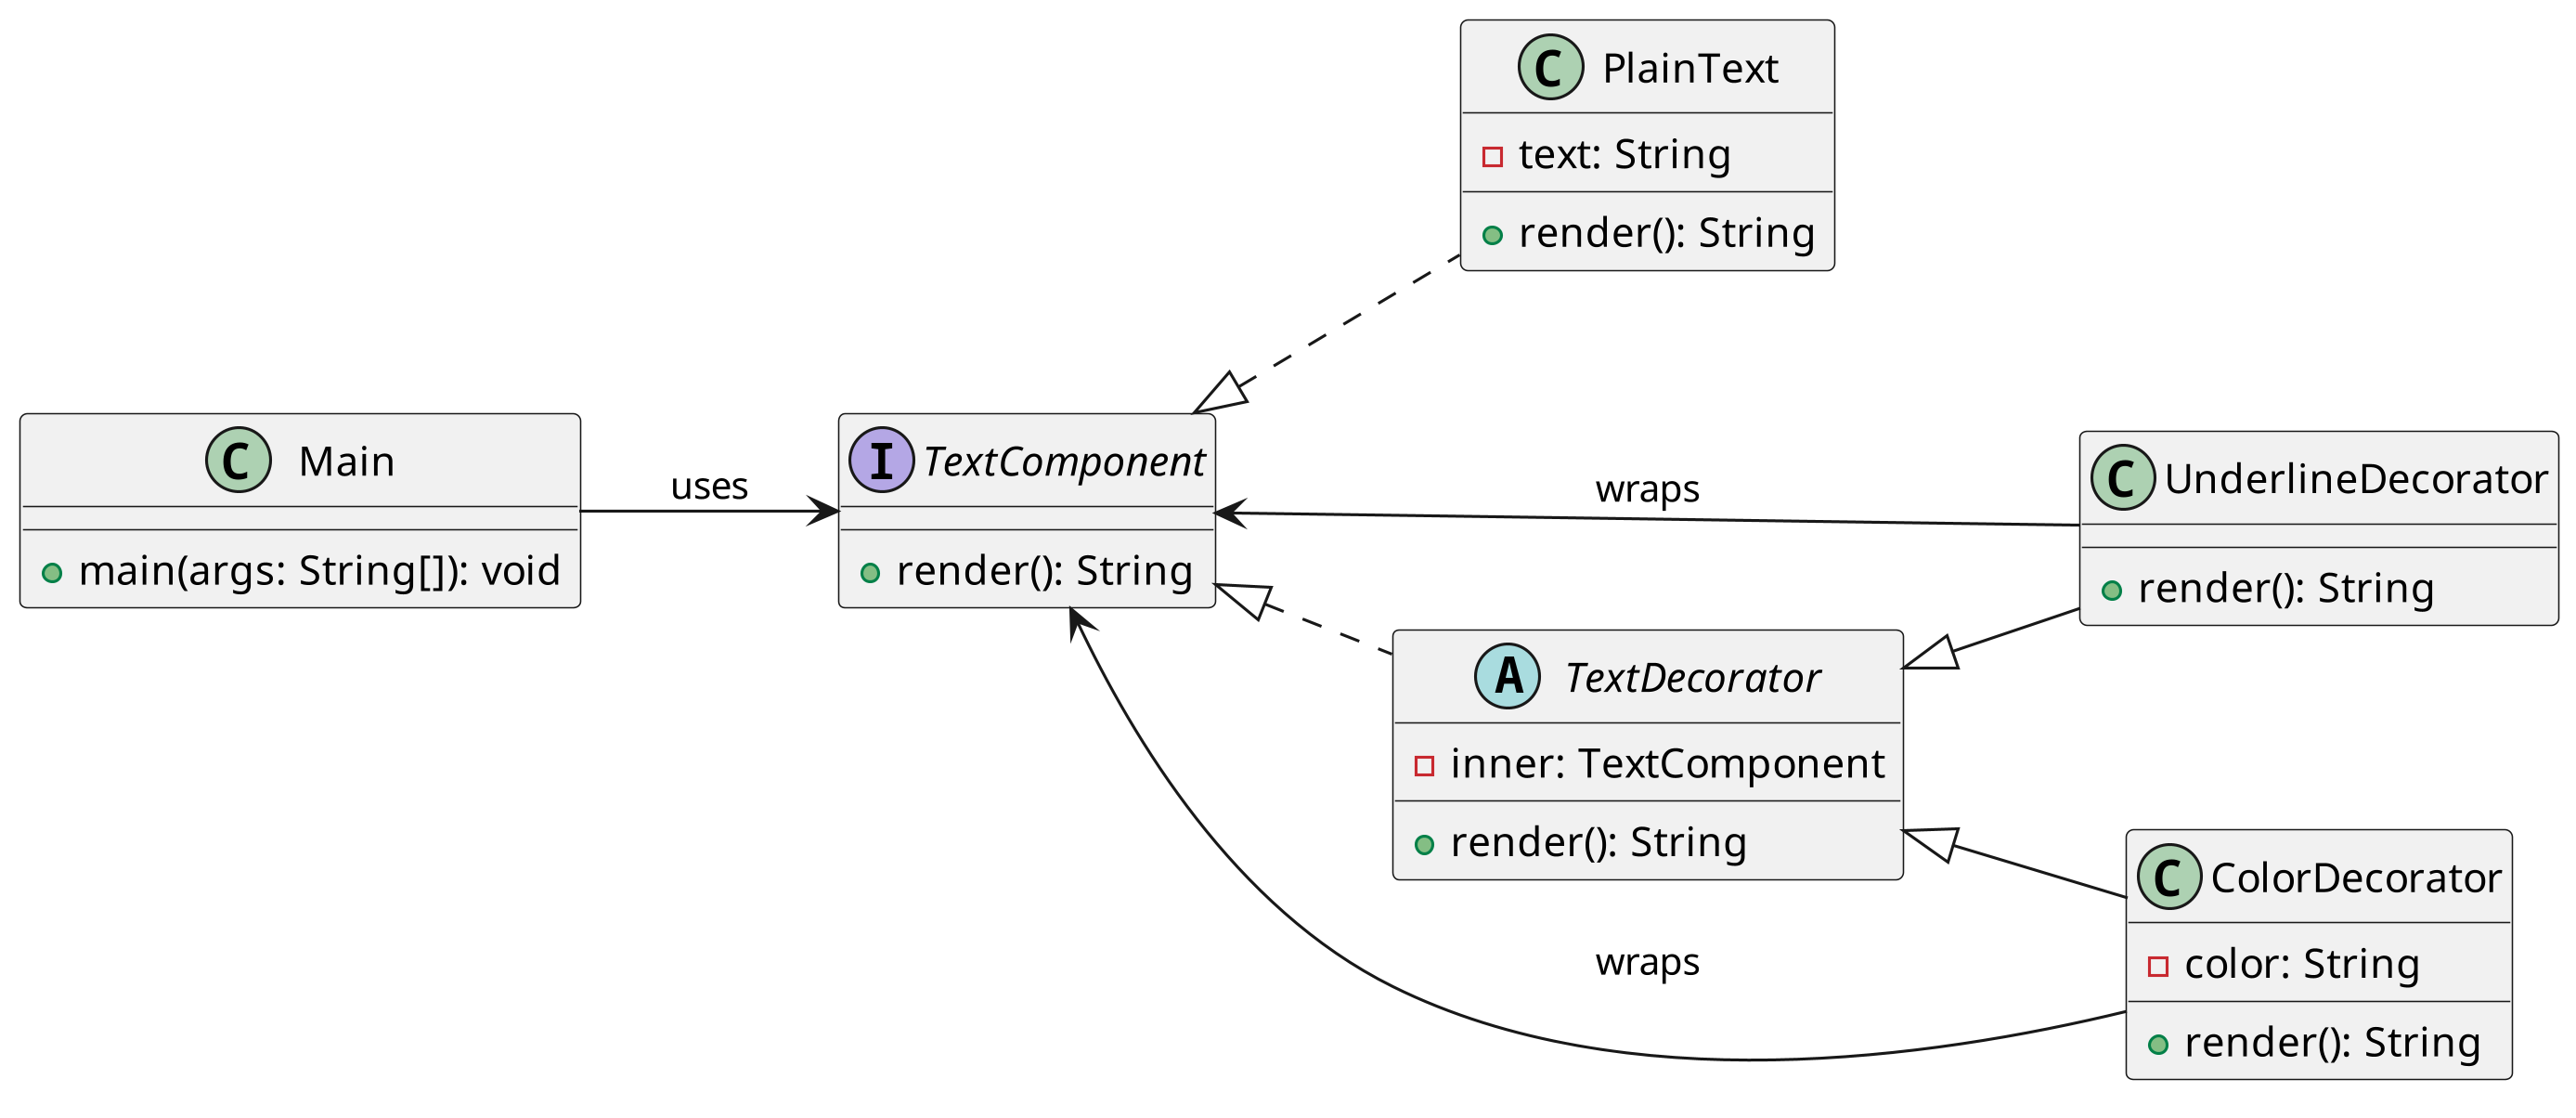
\includegraphics[width=0\textwidth]{../figures/out/decorator.png}
	\caption{Struktur Pola Decorator}
	\label{fig:decorator}
\end{figure}

Contoh berikut mengimplementasikan pola \textit{Decorator} untuk menghias teks sederhana dengan fitur tambahan seperti menambahkan garis bawah dan warna:

\begin{lstlisting}[style=JavaStyle, caption={Komponen Dasar: TextComponent}, label={lst:decorator-component}]
	public interface TextComponent {
		String render();
	}
\end{lstlisting}

\begin{lstlisting}[style=JavaStyle, caption={Komponen Konkret: PlainText}, label={lst:decorator-plaintext}]
	public class PlainText implements TextComponent {
		private String text;
		
		public PlainText(String text) {
			this.text = text;
		}
		
		@Override
		public String render() {
			return text;
		}
	}
\end{lstlisting}

\begin{lstlisting}[style=JavaStyle, caption={Decorator Abstrak: TextDecorator}, label={lst:decorator-decorator}]
	public abstract class TextDecorator implements TextComponent {
		protected TextComponent inner;
		
		public TextDecorator(TextComponent inner) {
			this.inner = inner;
		}
		
		public abstract String render();
	}
\end{lstlisting}

\begin{lstlisting}[style=JavaStyle, caption={Decorator Konkret: UnderlineDecorator}, label={lst:decorator-underline}]
	public class UnderlineDecorator extends TextDecorator {
		public UnderlineDecorator(TextComponent inner) {
			super(inner);
		}
		
		@Override
		public String render() {
			return "<u>" + inner.render() + "</u>";
		}
	}
\end{lstlisting}

\begin{lstlisting}[style=JavaStyle, caption={Decorator Konkret: ColorDecorator}, label={lst:decorator-color}]
	public class ColorDecorator extends TextDecorator {
		private String color;
		
		public ColorDecorator(TextComponent inner, String color) {
			super(inner);
			this.color = color;
		}
		
		@Override
		public String render() {
			return "<span style='color:" + color + "'>" + inner.render() + "</span>";
		}
	}
\end{lstlisting}

\begin{lstlisting}[style=JavaStyle, caption={Client: Penggunaan Decorator}, label={lst:decorator-main}]
	public class Main {
		public static void main(String[] args) {
			TextComponent text = new PlainText("Hello, Decorator!");
			TextComponent decorated = new ColorDecorator(new UnderlineDecorator(text), "blue");
			
			System.out.println(decorated.render());
		}
	}
\end{lstlisting}

Pada contoh di atas:
\begin{itemize}
	\item Objek \texttt{PlainText} adalah komponen dasar yang menyimpan string.
	\item Kelas \texttt{TextDecorator} adalah kelas abstrak yang menjadi dasar semua decorator.
	\item \texttt{UnderlineDecorator} menambahkan tag HTML \texttt{<u>} untuk memberikan efek garis bawah.
	\item \texttt{ColorDecorator} membungkus output dalam tag \texttt{<span>} dengan atribut warna.
	\item Objek dihias secara bertingkat: \texttt{UnderlineDecorator} membungkus \texttt{PlainText}, lalu \texttt{ColorDecorator} membungkus hasilnya.
\end{itemize}

Output dari program di atas adalah:
\begin{verbatim}
	<span style='color:blue'><u>Hello, Decorator!</u></span>
\end{verbatim}

Contoh ini menunjukkan fleksibilitas pola Decorator dalam membangun perilaku tambahan tanpa harus memodifikasi kelas utama, serta kemampuan untuk menggabungkan berbagai dekorasi dengan cara yang modular dan dinamis.



\section{Bridge}

\subsection{Tujuan dan Konteks Penggunaan}

Pola \textit{Bridge} merupakan pola struktural yang dirancang untuk memisahkan abstraksi dari implementasinya sehingga keduanya dapat dikembangkan secara independen. Pola ini sangat berguna dalam sistem yang memiliki banyak variasi dalam dua dimensi yang berbeda, misalnya: berbagai jenis bentuk (\textit{abstraction}) dan berbagai jenis cara menggambar bentuk tersebut (\textit{implementation}). Dengan pola ini, kita dapat menghindari kombinasi kelas yang meledak akibat pewarisan ganda yang tidak efisien.

Tujuan utama dari pola Bridge adalah untuk:
\begin{itemize}
	\item Menghindari pewarisan hirarki yang dalam dan rumit.
	\item Memisahkan logika level tinggi (abstraksi) dari detail teknis implementasinya.
	\item Mendukung perluasan fitur baik di sisi abstraksi maupun implementasi secara mandiri.
\end{itemize}

Pola ini terdiri dari dua hierarki terpisah:
\begin{enumerate}
	\item \textbf{Abstraction:} Merupakan antarmuka utama atau logika bisnis yang digunakan oleh klien. Kelas ini menyimpan referensi ke \texttt{Implementor}.
	\item \textbf{Implementor:} Berisi antarmuka atau kelas dasar yang mendefinisikan metode-metode yang akan diimplementasikan secara konkret.
\end{enumerate}

Bridge sangat sesuai digunakan ketika:
\begin{itemize}
	\item Terdapat dua dimensi perubahan yang perlu dikelola secara independen, seperti jenis dokumen dan metode penyimpanan (PDF, DOCX, HTML).
	\item Sistem membutuhkan fleksibilitas tinggi terhadap perubahan struktur internal tanpa memengaruhi antarmuka eksternal.
	\item Diperlukan arsitektur yang scalable dan modular untuk menangani kombinasi objek dalam jumlah besar.
\end{itemize}

Contoh klasik dari penggunaan Bridge adalah dalam sistem rendering grafis. Misalnya, bentuk geometris seperti \texttt{Circle}, \texttt{Rectangle}, dan \texttt{Triangle} dapat digambarkan di berbagai platform seperti OpenGL, DirectX, atau canvas HTML. Dengan pola Bridge, kita tidak perlu membuat subclass untuk setiap kombinasi bentuk dan platform, cukup memisahkan hierarki bentuk dari hierarki rendering.

Bridge juga banyak digunakan dalam sistem operasi (untuk memisahkan logika aplikasi dan implementasi platform), sistem kendali perangkat keras, serta antarmuka pengguna multiplatform.

Dengan pendekatan ini, sistem menjadi lebih mudah dikembangkan, diuji, dan dirawat, karena perubahan pada satu sisi (misalnya implementasi rendering) tidak berdampak langsung pada sisi lain (misalnya jenis bentuk yang digambar).

\subsection{Contoh Kasus Penggunaan}

Pola \textit{Bridge} sangat berguna dalam situasi di mana terdapat dua dimensi atau lebih yang berubah secara independen. Dengan memisahkan abstraksi dan implementasi ke dalam hierarki yang berbeda, pola ini menghindari duplikasi kode yang berlebihan dan membuat sistem lebih fleksibel serta mudah diperluas.

Salah satu contoh nyata adalah dalam sistem penggambaran bentuk (\textit{shape rendering}). Misalnya, kita memiliki berbagai jenis bentuk seperti \texttt{Circle}, \texttt{Rectangle}, dan \texttt{Triangle}, serta berbagai cara untuk menggambar bentuk tersebut, seperti menggunakan OpenGL, DirectX, atau HTML Canvas. Tanpa pola Bridge, kita perlu membuat subclass untuk setiap kombinasi, seperti \texttt{CircleWithOpenGL}, \texttt{CircleWithDirectX}, dan seterusnya. Hal ini akan menyebabkan ledakan jumlah kelas. Dengan Bridge, bentuk dan renderer dikelola dalam hierarki terpisah dan dihubungkan melalui komposisi, bukan pewarisan.

Contoh lainnya adalah dalam pengembangan aplikasi lintas platform, misalnya sebuah aplikasi UI yang berjalan di Windows, macOS, dan Linux. Komponen abstrak seperti \texttt{Window}, \texttt{Button}, atau \texttt{Dialog} dapat dipisahkan dari implementasi platformnya seperti \texttt{WinAPI}, \texttt{GTK}, atau \texttt{Qt}. Kelas \texttt{Window} akan berisi logika umum untuk menampilkan jendela, sedangkan kelas implementasi platform akan menangani detail rendering spesifik dari sistem operasi terkait.

Dalam sistem penyimpanan dokumen, pola Bridge dapat digunakan untuk memisahkan jenis dokumen (seperti \texttt{Invoice}, \texttt{Report}, \texttt{Letter}) dari cara penyimpanannya (seperti \texttt{DatabaseStorage}, \texttt{FileSystemStorage}, atau \texttt{CloudStorage}). Setiap jenis dokumen dapat memilih metode penyimpanan yang berbeda tanpa perlu membuat subclass baru untuk setiap kombinasi dokumen dan metode penyimpanan.

\textbf{Contoh dalam praktik:}
\begin{itemize}
	\item Dalam framework game, entitas seperti \texttt{Enemy} atau \texttt{NPC} dapat dipisahkan dari logika AI mereka. Abstraksi menangani perilaku umum, sementara implementor menangani strategi AI yang spesifik.
	\item Dalam sistem notifikasi, \texttt{Notification} adalah abstraksi dan dapat dikirim melalui berbagai saluran (\texttt{EmailSender}, \texttt{SMSSender}, \texttt{PushNotificationSender}) sebagai implementor.
	\item Dalam perangkat lunak multimedia, komponen \texttt{MediaPlayer} dapat memutar berbagai jenis media (video/audio), sementara decoding dilakukan oleh implementasi yang berbeda seperti \texttt{MP4Decoder}, \texttt{MKVDecoder}, atau \texttt{MP3Decoder}.
\end{itemize}

Dengan menggunakan pola Bridge, sistem menjadi lebih modular dan dapat dikembangkan dengan lebih mudah karena masing-masing dimensi variasi dapat ditangani secara terpisah dan digabungkan secara fleksibel saat runtime.

\subsection{Kelebihan dan Kekurangan}

Pola \textit{Bridge} memberikan sejumlah manfaat penting dalam pengembangan perangkat lunak yang kompleks dan berskala besar, terutama ketika menghadapi kebutuhan perluasan fitur dalam dua atau lebih dimensi. Namun, seperti pola desain lainnya, penerapannya juga memiliki beberapa potensi kelemahan yang perlu dipertimbangkan secara cermat.

\textbf{Kelebihan:}
\begin{itemize}
	\item \textbf{Memisahkan abstraksi dari implementasi:} Bridge memungkinkan abstraksi dan implementasi dikembangkan secara terpisah tanpa saling bergantung langsung. Hal ini memungkinkan fleksibilitas lebih tinggi dalam pengembangan dan pemeliharaan sistem.
	
	\item \textbf{Mendukung perluasan multidimensi:} Saat terdapat dua dimensi perubahan (misalnya: jenis perangkat dan jenis antarmuka, atau jenis bentuk dan jenis renderer), Bridge mencegah ledakan kombinasi kelas akibat pewarisan konvensional.
	
	\item \textbf{Mendukung prinsip Open/Closed dan Single Responsibility:} Perubahan pada bagian implementasi tidak memengaruhi abstraksi, dan sebaliknya. Hal ini sejalan dengan prinsip desain yang baik dalam pengembangan perangkat lunak.
	
	\item \textbf{Meningkatkan modularitas dan keterujian:} Karena komponen logika dan teknis dipisahkan, pengujian dapat dilakukan secara independen pada masing-masing hierarki tanpa harus membuat objek penuh dengan semua dependensi.
	
	\item \textbf{Mempermudah adopsi teknologi baru:} Jika ada perubahan platform, perangkat, atau metode implementasi (seperti renderer baru atau protokol komunikasi baru), perubahan dapat dilakukan hanya pada implementor tanpa menyentuh kode abstraksi.
\end{itemize}

\textbf{Kekurangan:}
\begin{itemize}
	\item \textbf{Meningkatkan kompleksitas struktur kode:} Struktur tambahan seperti antarmuka implementor, abstraksi, dan hubungan komposisi dapat membuat kode lebih kompleks dibanding pewarisan langsung dalam kasus yang sederhana.
	
	\item \textbf{Sulit dipahami oleh pengembang pemula:} Pola ini memperkenalkan abstraksi ganda yang tidak langsung terlihat dalam alur eksekusi program, sehingga memerlukan pemahaman konsep desain yang lebih matang.
	
	\item \textbf{Overengineering untuk kasus sederhana:} Jika sistem hanya memiliki satu dimensi perubahan atau variasi yang terbatas, penerapan Bridge dapat dianggap berlebihan dan justru menghambat produktivitas.
	
	\item \textbf{Pemeliharaan struktur ganda:} Karena ada dua hierarki yang berkembang secara paralel (abstraksi dan implementasi), pemeliharaan dan dokumentasi memerlukan konsistensi tambahan untuk mencegah ketidaksesuaian antar hierarki.
	
	\item \textbf{Potensi penyalahgunaan inheritance dan delegation:} Jika tidak dirancang dengan baik, hubungan antara abstraksi dan implementor dapat menjadi tidak jelas, dan pengguna dapat tergoda untuk menambahkan logika implementasi ke dalam abstraksi atau sebaliknya, melanggar pemisahan tanggung jawab.
\end{itemize}

Secara keseluruhan, pola \textit{Bridge} sangat efektif ketika sistem memiliki kombinasi dimensi variasi yang berkembang secara independen. Namun, penerapannya sebaiknya dilakukan ketika manfaat pemisahan benar-benar dibutuhkan, agar tidak menambah beban struktural secara tidak perlu pada sistem yang sebenarnya sederhana.

\subsection{Implementasi dalam Java}

Implementasi pola \textit{Bridge} dalam Java melibatkan dua hierarki yang terpisah namun terhubung melalui komposisi: hierarki abstraksi dan hierarki implementasi. Abstraksi bertanggung jawab atas logika tingkat tinggi yang digunakan oleh klien, sedangkan implementasi berisi detail teknis spesifik yang dapat divariasikan.

Gambar~\ref{fig:bridge} memperlihatkan struktur umum dari pola Bridge. Kelas \texttt{Abstraction} memiliki referensi ke objek bertipe \texttt{Implementor}, dan semua metode dari \texttt{Abstraction} akan didelegasikan ke \texttt{Implementor} sesuai kebutuhan. Dengan struktur ini, pengembang dapat menambahkan subclass baru pada salah satu hierarki tanpa harus menyentuh yang lain.

\begin{figure}[h]
	\centering
	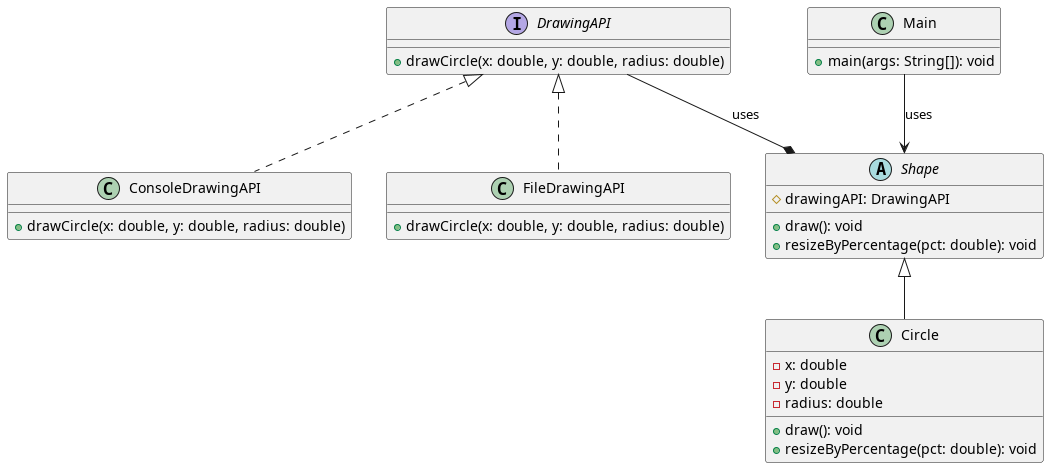
\includegraphics[width=\textwidth]{../figures/out/bridge.png}
	\caption{Struktur Pola Bridge}
	\label{fig:bridge}
\end{figure}

Contoh berikut menggambarkan bagaimana pola Bridge digunakan untuk menggambar bentuk (seperti lingkaran) menggunakan dua implementasi berbeda: melalui konsol dan melalui file.

\begin{lstlisting}[style=JavaStyle, caption={Implementor: DrawingAPI}, label={lst:bridge-api}]
	public interface DrawingAPI {
		void drawCircle(double x, double y, double radius);
	}
\end{lstlisting}

\begin{lstlisting}[style=JavaStyle, caption={Implementasi Konkret: ConsoleDrawingAPI}, label={lst:bridge-api-console}]
	public class ConsoleDrawingAPI implements DrawingAPI {
		@Override
		public void drawCircle(double x, double y, double radius) {
			System.out.println("Console: Drawing circle at (" + x + "," + y + ") with radius " + radius);
		}
	}
\end{lstlisting}

\begin{lstlisting}[style=JavaStyle, caption={Implementasi Konkret: FileDrawingAPI}, label={lst:bridge-api-file}]
	public class FileDrawingAPI implements DrawingAPI {
		@Override
		public void drawCircle(double x, double y, double radius) {
			System.out.println("File: Writing 'Circle (" + x + "," + y + ") radius " + radius + "' to file.");
			// Simulasi penulisan ke file
		}
	}
\end{lstlisting}

\begin{lstlisting}[style=JavaStyle, caption={Abstraksi: Shape}, label={lst:bridge-abstraction}]
	public abstract class Shape {
		protected DrawingAPI drawingAPI;
		
		protected Shape(DrawingAPI drawingAPI) {
			this.drawingAPI = drawingAPI;
		}
		
		public abstract void draw();           // low-level
		public abstract void resizeByPercentage(double pct);  // high-level
	}
\end{lstlisting}

\begin{lstlisting}[style=JavaStyle, caption={Abstraksi Konkret: Circle}, label={lst:bridge-circle}]
	public class Circle extends Shape {
		private double x, y, radius;
		
		public Circle(double x, double y, double radius, DrawingAPI drawingAPI) {
			super(drawingAPI);
			this.x = x;
			this.y = y;
			this.radius = radius;
		}
		
		@Override
		public void draw() {
			drawingAPI.drawCircle(x, y, radius);
		}
		
		@Override
		public void resizeByPercentage(double pct) {
			radius *= (1.0 + pct / 100.0);
		}
	}
\end{lstlisting}

\begin{lstlisting}[style=JavaStyle, caption={Client: Menggunakan Bridge Pattern}, label={lst:bridge-main}]
	public class Main {
		public static void main(String[] args) {
			Shape circle1 = new Circle(1, 2, 3, new ConsoleDrawingAPI());
			Shape circle2 = new Circle(5, 7, 10, new FileDrawingAPI());
			
			circle1.draw(); // Output ke konsol
			circle2.draw(); // Simulasi output ke file
		}
	}
\end{lstlisting}

Pada contoh di atas:
\begin{itemize}
	\item Antarmuka \texttt{DrawingAPI} mendefinisikan operasi dasar untuk menggambar lingkaran.
	\item Dua implementasi berbeda (\texttt{ConsoleDrawingAPI} dan \texttt{FileDrawingAPI}) menunjukkan dua teknik rendering.
	\item Kelas \texttt{Shape} bertindak sebagai abstraksi, dan menyimpan referensi ke \texttt{DrawingAPI}.
	\item Kelas \texttt{Circle} sebagai turunan dari \texttt{Shape} menggunakan API yang disuntikkan untuk menggambar lingkaran sesuai cara yang dipilih (konsol atau file).
\end{itemize}

Dengan pendekatan ini, pengembang dapat menambahkan jenis \texttt{Shape} baru (misalnya \texttt{Rectangle}, \texttt{Triangle}) tanpa mengubah kode API, dan sebaliknya menambahkan renderer baru tanpa menyentuh kelas bentuk. Pola Bridge ini memaksimalkan skalabilitas dan fleksibilitas sistem dengan struktur yang tetap modular dan mudah diuji.



\section{Composite}

\subsection{Tujuan dan Konteks Penggunaan}

Pola \textit{Composite} adalah salah satu pola struktural yang bertujuan untuk menangani struktur hierarki objek, di mana klien dapat memperlakukan objek tunggal (individu) dan objek yang terdiri dari kumpulan objek lain (komposit) dengan cara yang sama. Dengan pola ini, struktur pohon (tree structure) seperti file system, struktur dokumen, dan antarmuka pengguna dapat dimodelkan secara elegan dan fleksibel.

Tujuan utama dari pola \textit{Composite} adalah untuk:
\begin{itemize}
	\item Menyatukan objek sederhana dan objek kompleks ke dalam struktur hirarkis yang konsisten.
	\item Memungkinkan operasi dilakukan secara rekursif pada struktur komposit.
	\item Menyederhanakan logika klien dengan cara menyatukan antarmuka objek individual dan objek komposit.
\end{itemize}

Pola ini terdiri dari tiga komponen utama:
\begin{enumerate}
	\item \textbf{Component:} Antarmuka atau kelas abstrak yang mendefinisikan operasi umum yang dapat dilakukan pada objek, baik leaf maupun composite.
	\item \textbf{Leaf:} Objek individu dalam struktur yang tidak memiliki anak.
	\item \textbf{Composite:} Objek yang dapat menyimpan satu atau lebih objek anak (baik \texttt{Leaf} maupun \texttt{Composite} lainnya) dan meneruskan operasi ke anak-anaknya.
\end{enumerate}

Pola Composite sangat sesuai digunakan dalam situasi berikut:
\begin{itemize}
	\item Ketika objek perlu disusun dalam bentuk pohon (tree) dan klien harus memperlakukan semua objek dalam struktur tersebut secara seragam.
	\item Saat pengoperasian terhadap elemen-elemen tunggal dan grup elemen memerlukan perlakuan yang konsisten (misalnya operasi \texttt{draw()}, \texttt{print()}, atau \texttt{calculate()}).
	\item Ketika sistem perlu menangani struktur data yang dapat berkembang secara dinamis dalam bentuk hierarki.
\end{itemize}

Contoh umum penggunaan Composite antara lain:
\begin{itemize}
	\item Struktur folder dan file dalam file system, di mana folder bisa berisi file atau folder lainnya.
	\item Elemen-elemen grafis dalam antarmuka pengguna seperti panel yang berisi tombol, label, dan elemen visual lainnya.
	\item Representasi struktur dokumen seperti dokumen HTML, XML, atau JSON, di mana tag dapat bersarang secara rekursif.
\end{itemize}

Dengan menerapkan pola Composite, sistem menjadi lebih fleksibel dalam memproses struktur data rekursif, dan kode klien dapat dibuat lebih bersih karena tidak perlu membedakan antara objek individu dan komposit.

\subsection{Contoh Kasus Penggunaan}

Pola \textit{Composite} sangat efektif dalam berbagai skenario di mana objek-objek perlu disusun dalam bentuk struktur hierarkis, dan operasi yang sama harus diterapkan baik pada objek individual maupun pada grup objek. Dengan menyatukan antarmuka antara elemen sederhana dan elemen kompleks, klien dapat bekerja dengan semua elemen secara konsisten tanpa harus melakukan pengecekan tipe atau logika khusus.

Salah satu contoh paling umum adalah pada sistem berkas (\textit{file system}). Dalam struktur direktori komputer, terdapat dua jenis entitas: \texttt{File} dan \texttt{Directory}. File adalah elemen akhir yang menyimpan data, sedangkan Directory adalah struktur yang dapat berisi File maupun Directory lain (secara rekursif). Dengan menggunakan pola Composite, kelas \texttt{File} dan \texttt{Directory} dapat mengimplementasikan antarmuka yang sama, misalnya metode \texttt{getSize()} atau \texttt{printStructure()}, dan klien dapat memanggil metode ini tanpa harus mengetahui apakah objek tersebut adalah file atau folder.

Contoh lainnya adalah dalam antarmuka pengguna grafis (GUI). Sebuah jendela (window) dapat berisi berbagai komponen seperti \texttt{Button}, \texttt{TextField}, atau bahkan \texttt{Panel} lain yang juga berisi komponen tambahan. Dengan pola Composite, semua komponen ini dapat diperlakukan sebagai \texttt{UIComponent} dan diproses secara rekursif, misalnya saat melakukan perintah \texttt{render()}, \texttt{resize()}, atau \texttt{disable()}.

Dalam dunia bisnis, pola ini dapat diterapkan pada struktur organisasi. Misalnya, perusahaan terdiri dari berbagai divisi, dan masing-masing divisi memiliki departemen atau bahkan tim kerja. Tiap entitas ini, baik individu (karyawan) maupun grup (departemen, divisi), dapat mengimplementasikan antarmuka \texttt{OrganizationUnit} yang mendukung operasi seperti \texttt{printHierarchy()} atau \texttt{calculateTotalSalary()}.

\textbf{Contoh dalam praktik:}
\begin{itemize}
	\item Sistem manajemen proyek yang memiliki struktur tugas dan sub-tugas, di mana masing-masing tugas dapat memiliki durasi, status, atau penanggung jawab yang dapat dihitung secara agregat.
	\item Representasi struktur menu pada aplikasi desktop atau web, di mana setiap \texttt{MenuItem} bisa menjadi perintah tunggal atau submenu yang berisi item lainnya.
	\item Sistem kalkulasi biaya produksi di mana produk akhir merupakan komposit dari beberapa komponen, dan tiap komponen juga dapat terdiri dari sub-komponen lainnya.
\end{itemize}

Dengan pola Composite, operasi seperti perhitungan, pencetakan, atau manipulasi hierarki dapat diterapkan dengan cara rekursif dan seragam, menjadikan kode lebih bersih, modular, dan mudah dikembangkan.

\subsection{Kelebihan dan Kekurangan}

Pola \textit{Composite} memberikan sejumlah keuntungan penting dalam pengembangan sistem yang memiliki struktur data hierarkis atau bersarang. Dengan menyatukan antarmuka antara objek individu dan objek komposit, pola ini menyederhanakan logika klien dan meningkatkan konsistensi pengolahan data. Namun, seperti pola desain lainnya, penerapan Composite juga memiliki beberapa kekurangan yang perlu diperhatikan.

\textbf{Kelebihan:}
\begin{itemize}
	\item \textbf{Menyederhanakan logika klien:} Klien dapat memperlakukan objek tunggal dan komposit dengan cara yang sama karena keduanya menggunakan antarmuka yang seragam. Hal ini mengurangi kebutuhan logika bersyarat (seperti \texttt{instanceof}) untuk membedakan jenis objek.
	
	\item \textbf{Mendukung struktur rekursif:} Composite sangat cocok untuk memodelkan struktur pohon yang bersifat rekursif, seperti folder dalam sistem file, struktur organisasi, atau struktur komponen dalam antarmuka pengguna.
	
	\item \textbf{Mudah diperluas:} Penambahan jenis elemen baru (baik leaf maupun composite) dapat dilakukan tanpa mengubah kode klien atau struktur yang sudah ada, sehingga mendukung prinsip Open/Closed.
	
	\item \textbf{Meningkatkan modularitas dan reusabilitas:} Dengan memisahkan objek menjadi bagian-bagian komposit dan leaf yang terdefinisi dengan jelas, sistem menjadi lebih modular dan bagian-bagiannya dapat digunakan kembali di konteks lain.
	
	\item \textbf{Mendukung operasi agregasi:} Operasi seperti total harga, durasi, atau ukuran dapat dihitung secara rekursif melalui struktur komposit, tanpa harus mengetahui struktur detail dari masing-masing komponen.
\end{itemize}

\textbf{Kekurangan:}
\begin{itemize}
	\item \textbf{Sulit membatasi jenis objek anak:} Karena leaf dan composite memiliki antarmuka yang sama, tidak ada mekanisme bawaan untuk mencegah penambahan anak ke objek leaf, kecuali melalui validasi eksplisit.
	
	\item \textbf{Overhead struktur tambahan:} Untuk kasus sederhana, penggunaan struktur komposit bisa dianggap berlebihan dan justru menambah kompleksitas serta konsumsi memori yang tidak diperlukan.
	
	\item \textbf{Menyembunyikan perbedaan antara leaf dan composite:} Abstraksi yang menyatukan antarmuka dapat menyebabkan klien kehilangan informasi penting tentang struktur internal objek, sehingga dapat mengaburkan pemahaman terhadap hierarki.
	
	\item \textbf{Kesulitan debugging dan pelacakan:} Ketika struktur komposit sangat dalam atau kompleks, pelacakan bug atau analisis perilaku sistem bisa menjadi lebih sulit karena prosesnya tersembunyi dalam banyak level rekursif.
	
	\item \textbf{Peningkatan kompleksitas pengelolaan dependensi:} Dalam struktur yang dinamis, menjaga konsistensi antar node (seperti referensi induk atau sinkronisasi status) memerlukan perhatian khusus dan potensi peningkatan beban logika.
\end{itemize}

Secara keseluruhan, pola \textit{Composite} sangat efektif dalam membangun sistem yang bersifat hierarkis dan berulang. Namun, seperti semua pola desain, penggunaannya harus disesuaikan dengan kebutuhan dan kompleksitas domain, agar tidak menimbulkan beban struktural yang tidak perlu.

\subsection{Implementasi dalam Java}

Implementasi pola \textit{Composite} dalam Java melibatkan pembuatan antarmuka atau kelas abstrak yang menyatukan perilaku dari objek individu (\texttt{Leaf}) dan objek gabungan (\texttt{Composite}). Dengan pendekatan ini, struktur pohon dapat dibentuk, dan klien dapat menggunakan objek secara rekursif tanpa membedakan apakah objek tersebut merupakan elemen tunggal atau komposit.

Gambar~\ref{fig:composite} menunjukkan struktur pola \textit{Composite} dalam bentuk diagram UML. Kelas \texttt{FileSystemNode} merupakan antarmuka dasar yang diimplementasikan oleh kelas \texttt{File} dan \texttt{Directory}. Kelas \texttt{Directory} bertindak sebagai komposit yang dapat berisi daftar objek \texttt{FileSystemNode}, baik berupa \texttt{File} maupun \texttt{Directory} lainnya, membentuk struktur pohon yang dapat diproses secara rekursif.

\begin{figure}[h]
	\centering
	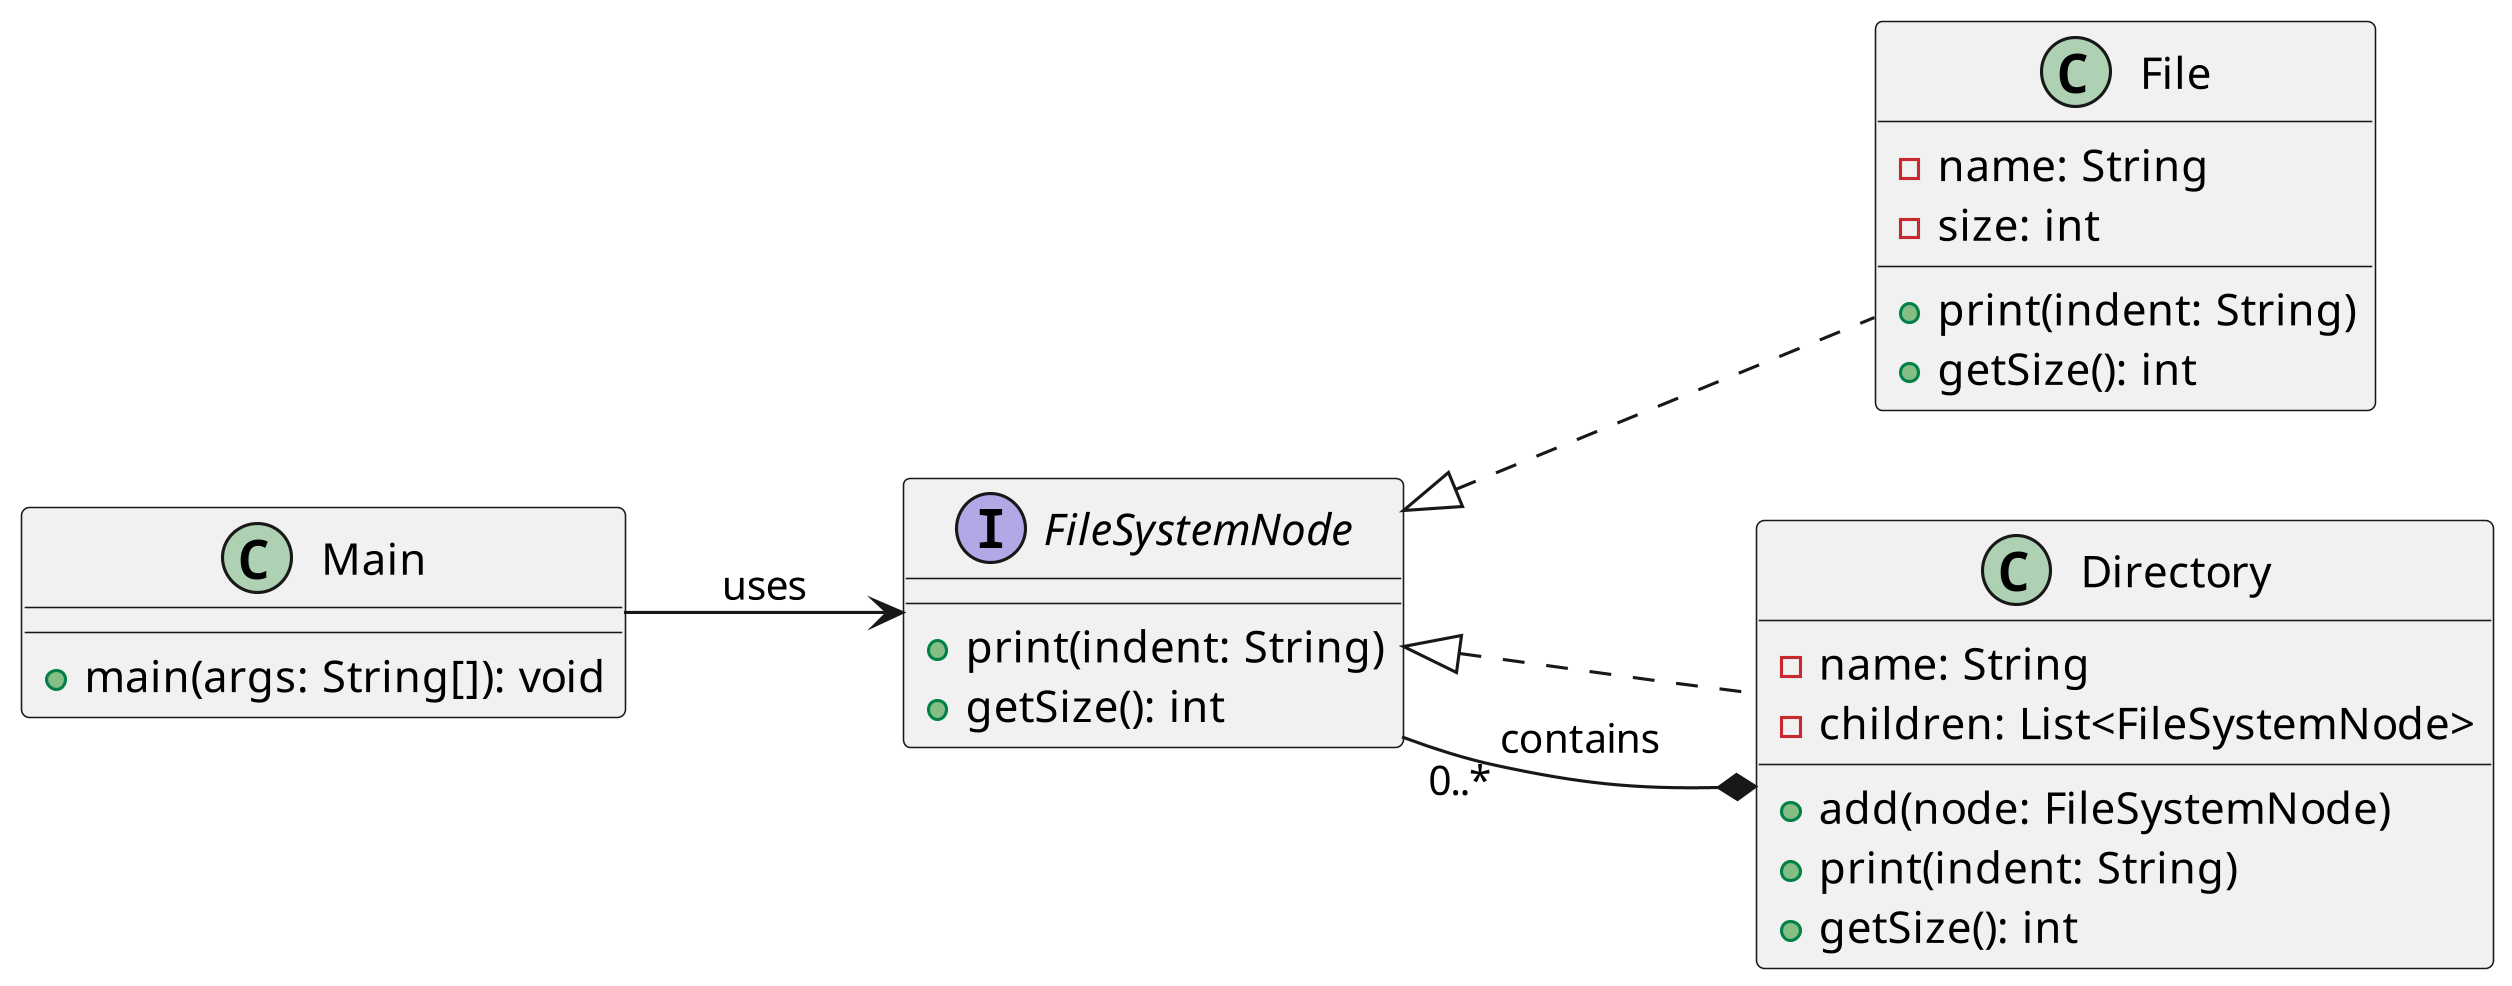
\includegraphics[width=\textwidth]{../figures/out/composite.png}
	\caption{Struktur Pola Composite}
	\label{fig:composite}
\end{figure}

Contoh berikut menunjukkan implementasi sederhana dari sistem file, di mana \texttt{File} merupakan leaf dan \texttt{Directory} merupakan composite yang dapat berisi file maupun direktori lain.

\begin{lstlisting}[style=JavaStyle, caption={Component: FileSystemNode}, label={lst:composite-interface}]
	public interface FileSystemNode {
		void print(String indent);
		int getSize(); // ukuran dalam kilobyte
	}
\end{lstlisting}

\begin{lstlisting}[style=JavaStyle, caption={Leaf: File}, label={lst:composite-leaf}]
	public class File implements FileSystemNode {
		private String name;
		private int size;
		
		public File(String name, int size) {
			this.name = name;
			this.size = size;
		}
		
		@Override
		public void print(String indent) {
			System.out.println(indent + "- File: " + name + " (" + size + "KB)");
		}
		
		@Override
		public int getSize() {
			return size;
		}
	}
\end{lstlisting}

\begin{lstlisting}[style=JavaStyle, caption={Composite: Directory}, label={lst:composite-composite}]
	import java.util.ArrayList;
	import java.util.List;
	
	public class Directory implements FileSystemNode {
		private String name;
		private List<FileSystemNode> children = new ArrayList<>();
		
		public Directory(String name) {
			this.name = name;
		}
		
		public void add(FileSystemNode node) {
			children.add(node);
		}
		
		@Override
		public void print(String indent) {
			System.out.println(indent + "+ Directory: " + name);
			for (FileSystemNode child : children) {
				child.print(indent + "  ");
			}
		}
		
		@Override
		public int getSize() {
			int totalSize = 0;
			for (FileSystemNode child : children) {
				totalSize += child.getSize();
			}
			return totalSize;
		}
	}
\end{lstlisting}

\begin{lstlisting}[style=JavaStyle, caption={Client: Struktur File}, label={lst:composite-main}]
	public class Main {
		public static void main(String[] args) {
			File file1 = new File("resume.pdf", 120);
			File file2 = new File("budget.xlsx", 200);
			File file3 = new File("notes.txt", 30);
			
			Directory docs = new Directory("Documents");
			docs.add(file1);
			docs.add(file2);
			
			Directory root = new Directory("Home");
			root.add(docs);
			root.add(file3);
			
			root.print(""); // cetak struktur
			System.out.println("Total size: " + root.getSize() + "KB");
		}
	}
\end{lstlisting}

Penjelasan dari struktur kode:
\begin{itemize}
	\item \texttt{FileSystemNode} adalah antarmuka komponen yang mendefinisikan operasi \texttt{print()} dan \texttt{getSize()}.
	\item \texttt{File} adalah objek \texttt{Leaf} yang tidak memiliki anak dan hanya mengembalikan ukuran dirinya sendiri.
	\item \texttt{Directory} adalah \texttt{Composite} yang menyimpan koleksi \texttt{FileSystemNode} lain, memungkinkan penyusunan struktur rekursif.
	\item \texttt{Main} menunjukkan bagaimana objek-objek ini diorganisasi ke dalam struktur pohon, dan operasi dapat dipanggil secara seragam.
\end{itemize}

Dengan pendekatan ini, struktur file yang kompleks dapat dibangun dan dikelola secara fleksibel. Klien tidak perlu mengetahui apakah sebuah node adalah file atau direktori, karena semua node mengikuti antarmuka \texttt{FileSystemNode}. Pendekatan ini mempermudah pengembangan fitur seperti perhitungan ukuran, pencarian file, atau pencetakan struktur folder secara rekursif.

Pola \textit{Composite} memungkinkan penambahan jenis node baru (misalnya, \texttt{SymbolicLink}) tanpa harus mengubah kode yang ada, karena semua node mengikuti kontrak yang sama.

\section{Kesimpulan}

Pola-pola struktural seperti \textit{Adapter}, \textit{Decorator}, \textit{Bridge}, dan \textit{Composite} memberikan solusi desain yang elegan untuk mengelola hubungan antar kelas dan objek dalam sistem perangkat lunak. Pola \textit{Adapter} memungkinkan integrasi antara antarmuka yang tidak kompatibel, \textit{Decorator} menyediakan mekanisme fleksibel untuk menambahkan tanggung jawab pada objek secara dinamis, \textit{Bridge} memisahkan abstraksi dari implementasinya agar keduanya dapat berkembang secara independen, dan \textit{Composite} memungkinkan penyusunan objek ke dalam struktur hierarkis yang dapat diperlakukan secara seragam oleh klien.

Dengan menerapkan pola-pola ini secara tepat, pengembang dapat membangun sistem yang lebih modular, dapat diperluas, dan mudah dipelihara. Masing-masing pola memiliki keunggulan dan kelemahan yang harus dipertimbangkan berdasarkan kebutuhan spesifik arsitektur dan kompleksitas proyek. Pemahaman mendalam terhadap pola struktural ini merupakan fondasi penting dalam rekayasa perangkat lunak berorientasi objek untuk menghasilkan desain yang bersih, terstruktur, dan scalable.

